\documentclass[
  a4paper,
  abstracton,
  twocolumn,
  emulatestandardclasses
]{scrartcl}

\usepackage[english]{babel}
\usepackage{xcolor}
\usepackage{authblk}
\usepackage{amsthm}
\usepackage{amsmath}
\usepackage{amssymb}
\usepackage{physics}
\usepackage{csquotes}
\usepackage{paralist}
\usepackage[
  backend=biber,
  sorting=none
]{biblatex}
\usepackage{graphicx}
\usepackage[hidelinks]{hyperref}
\usepackage{cleveref}
\usepackage[binary-units]{siunitx}
\usepackage[margin=14pt]{caption}
\usepackage{booktabs}
\usepackage{pgfplots}
\usepackage{adjustbox}

\title{MRI to CT Translation with GANs}
\author[1]{Bodo Kaiser}
\author[2]{Shadi Albarqouni}
\affil[1]{\textit{bodo.kaiser@physik.uni-muenchen.de}}
\affil[2]{\textit{shadi.albarqouni@tum.de}}

\pgfplotsset{compat=newest}
\addbibresource{literature.bib}

\begin{document}

\makeatletter
\twocolumn[
	\begin{@twocolumnfalse} 
		\maketitle
		\begin{abstract}
  Lorem ipsum dolor sit amet, consectetuer adipiscing elit. Aenean commodo
  ligula eget dolor. Aenean massa. Cum sociis natoque penatibus et magnis dis
  parturient montes, nascetur ridiculus mus. Donec quam felis, ultricies nec,
  pellentesque eu, pretium quis, sem. Nulla consequat massa quis enim. Donec
  pede justo, fringilla vel, aliquet nec, vulputate eget, arcu. In enim justo,
  rhoncus ut, imperdiet a, venenatis vitae, justo. Nullam dictum felis eu pede
  mollis pretium.
\end{abstract}

		\vspace{1em}
	\end{@twocolumnfalse}
]
\makeatother

\section{Introduction}

\gls{ct} and \gls{mri} are the main workhorses of todays clinical diagnosis
and cancer monitoring by revealing the inner organ conditions without surgery.
Inside the clinical framework \gls{mri} is the more informative and safer
modality~\cite{Hartwig09}. Instead of x-rays which are known to possess the
risk of provoking cancer inside the patient~\cite{Martin06}, \gls{mri} exploit
the magnetic properties of hydrogen nucleus and are not associated with any
health risks. Additionally \gls{mri} provides a much higher soft tissue. These
benefitial characteristics suggest that \gls{mri} supersdes \gls{ct} in the
long-term. One of many remaining obstacles is, however, the requirement of
\gls{ct} for image guided radiation therapy planning. Although \gls{mri} and
\gls{ct} differ significant in the applied physics, the high entropy inside
\gls{mri} data suggests the existence of a one directional mapping from
\gls{mri} to \gls{ct} space. With the recent advent of computer vision
techniques based on \gls{gan} we seem to close to find such a mapping.

\section{Related Work}

Since the early days of \gls{ct}, health manufacturer were attempted to reduce
radiation exposure in \gls{ct} scans by using, for instance, more sensible
detection electronics, and more sophisticated scanning sequences. Through the
growing availability of computing power we also find evermore computer vision
techniques being utilized, for example, in the enhancement of image quality of
low-dose \gls{ct}s~\cite{Xu12}. Altough these efforts have lead to an
impressive and steady evolution of the \gls{ct} apparatus, they still require
the patient to be irradiated nevertheless.
First approaches which dispense the radiation exposure, through the
computational transformation of \gls{mri} to \gls{ct}, relay on the
atlas-based transformations applied to \gls{mri} to predict \gls{ct}, see
Ref.~\cite{Hofmann08}. Further improvements thereto include, for instance,
random forests~\cite{Andreasen13}. Finally it has been shown that these
\gls{ct} prediction methods can in fact already replace physical \gls{ct}
for treatment planning~\cite{Andreasen2017}.
At the same time, we have seen an incredible progress with deep learning
techniques in computer science~\cite{LeCun15}. Recent efforts with \gls{gan}s,
see Ref.~\cite{Goodfellow14}, seem to be a promising path towards finding
a global optimum in training neural networks through the use of game theory.
Furthermore \gls{gan}s proved significant improvements over the former state
of art in the task of image to image translation~\cite{Isola16} but also the
generalization of three dimensional structures inside the so called latent
space~\cite{ZXFT16}.
Keeping this in mind, the medical computer vision community rapidly adapted
\gls{gan}s for their own specific tasks. In comparison to datasets common in
general computer vision, medical datasets typical comprise volumetric single
channel images with high bit depth. Bearing the challenge of \gls{ct} from
\gls{mri} prediction in mind, the expectations towards \gls{gan}s have been
lately shown increased performance to the previous approaches~\cite{Nie16}.
Yet, the full potential of \gls{gan}s have not been exhausted. For example,
it has been shown that \gls{gan}s are capable of being trained with
unregistered modalities~\cite{Wolterink17}.
Beside the enourmous breakthroughs made in medical computer vision we still
see a shortage in a reproducable comparison of recent methods with publicly
available data. Not to mention the open questions with regard to best
practices in choosing good \gls{gan} model parameters for the task of
\gls{ct} prediction which we hope to address in the subsequent sections.

\section{Method}

In the consecutive parts we discuss the parameters relevant for the conducted
experiments. This includes decisions we made for the setup as a whole
(dataset, pre processing) but also detail decisions regarding for example
the implementation of a specific model. The source code based on the
Tensorflow framework~\cite{tensorflow15} will be made available through
GitHub.

\subsection{Dataset and preprocessing}

We used the publicly available dataset from the \gls{RIRE} project~\cite{RIRE},
which contains multi modality data of about 19 patients from which a subset
of 17 patients have a complete pair of T1 weighted MR and CT volume.
\begin{figure}[h]
  \centering
  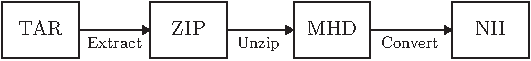
\includegraphics[width=\linewidth]{figure/conversion.pdf}
  \caption{Dataset conversion from \gls{mhd} to \gls{nifti} format.
	}\label{fig:conversion}
\end{figure}

We were able to co-register the modalities using \cite{SPM12} and the
highest interpolation order. In the same step we also resliced the volumes
to have a homogenous voxel size as the RIRE dataset has only a low resolution
in the sagittal plane.

Finally we used \cite{Nibabel} to load the aligned volumes and convert them
into Tensorflow's tfrecord format and split them into a validation set of
4 and a training set of 13 patients. Inside the tensorflow input pipeline
we normalized the value range of each volume to $[0,1]$. For two dimensional
models we padded the horizontal slices to $384\times384$. For three
dimensional models we used $260\times340\times360$ (Depth x Height x Width).

\subsection{Network}

As generative adversarial networks we decided to use pix2pix \cite{Isola16}
as it has already shown great results in the task of color image to image
translation and context-aware 3d synthesis \cite{Nie16} which uses a simpler
generator but accounts for 3d structures.

As convolutional encoder-decoder network we chose u-net \cite{Ronneberger15}
as it was able to compete with much larger models in the task of semantic
segmentation \cite{Badrinarayanan15}. Further our implementation of pix2pix
uses u-net as generator network, hence we are able to evaluate the impact
of the adversarial min-max approach.

Eventually we want to evaluate a new network and training approach novel to
medical computer vision \cite{Karras17}.

\subsubsection{U-Net}


\subsubsection{Pix2Pix}

\subsubsection{3D Synthesis}

\subsection{Losses}

\subsubsection{Distance Losses}

As norm losses we refer to the mean absolute error ($L1$ loss) and the
mean squared error ($L2$ loss).

\subsubsection{Gradient Losses}

The gradient (difference) loss is used in the framework of context-aware
3d synthesis \cite{Nie16} in addition to the norm loss.

\subsubsection{Signal Losses}

From signal processing PSNR, SSE...

\subsubsection{Adversarial Loss}

Least-squared adversarial loss, standard adversarial loss. BEGAN loss ?


\subsection{Augmentation}

\subsubsection{Random Crop}
\subsubsection{Rotation}
\subsubsection{Contast Adjustment}


\section{Result}


\printbibliography{}

\end{document}
